% !TEX TS-program = pdflatex
% !TEX encoding = UTF-8 Unicode

% This is a simple template for a LaTeX document using the "article" class.
% See "book", "report", "letter" for other types of document.
\documentclass[11pt,man]{article}
\usepackage{array}
\usepackage{color}
\usepackage[sort]{natbib}
\usepackage{amssymb}
\usepackage{amsmath}
\usepackage{amsfonts}
\usepackage{graphicx}
\usepackage{url}
\usepackage[font={small}]{caption, subfig}
\usepackage[vlined,ruled, noend,linesnumbered]{algorithm2e} 
\usepackage[margin=1in]{geometry}
\usepackage[T1]{fontenc}
\usepackage[utf8]{inputenc}
\usepackage{enumitem}
\usepackage{authblk}
\usepackage{tabularx}
\newcommand\numberthis{\addtocounter{equation}{1}\tag{\theequation}}

\definecolor{Orange}{rgb}{1,0.5,0}
\definecolor{Purple}{rgb}{1,0,1}
\definecolor{Green}{rgb}{0,1,0}
\definecolor{Red}{rgb}{1,0,0}

\newcommand{\todo}[1]{\textsf{\textbf{\textcolor{Red}{todo anyone: [[#1]]}}}}

\newcommand{\todoMatt}[1]{\textsf{\textbf{\textcolor{Orange}{todo Matt: [[#1]]}}}}
\newcommand{\todoKenny}[1]{\textsf{\textbf{\textcolor{Purple}{todo Kenny: [[#1]]}}}}
\newcommand{\todoWei}[1]{\textsf{\textbf{\textcolor{Green}{todo Wei: [[#1]]}}}}
\newcommand{\Expect}{{\rm I\kern-.3em E}}


\def\citeapos#1{\citeauthor{#1}'s (\citeyear{#1})}

\title{Using news media and Twitter to provide a quantitative overview of factors related to the outbreak, successes and failures of the "Arab Spring" }

\author[1]{Kenneth Joseph \thanks{\texttt{kjoseph@cs.cmu.edu}}}
\author[1]{Matthew Benigni \thanks{\texttt{mbenigni@cs.cmu.edu}}}
\author[1]{Wei Wei \thanks{\texttt{weiwei@cs.cmu.edu}}}
\author[1]{Kathleen M. Carley\thanks{\texttt{kathleen.carley@cs.cmu.edu}}}
\author[2]{Mia Bloom\thanks{\texttt{mia\_bloom@uml.edu}}}

\affil[1]{Computation, Organization and Society Program\\ Carnegie Mellon University\\ 5000 Forbes Ave. \\ Pittsburgh, PA, USA}
\affil[2]{Center for Terrorism and Security Studies\\ University of Massachusetts, Lowell\\ Lowell, MA, USA}


\begin{document}
\maketitle
\begin{abstract}
asdfsadf
\end{abstract}

\section{Introduction}

Story concepts:

how do discussions change over time and space in the arab spring?

this allows us to compare public focus and news focus

which drives which and how much

in intro: problems with count data, e.g. by showing diffrences in A, other biases

Work to do:

1. Fake data
	create 1 that is positive, does it recover
	random walk data

2. Stop word data
	top 25 nouns, 3 topics (minus man, woman, child, life, gov't)
	top 25 nouns, top 25 adjectives, 3 topics (minus above + young)
3. Re-estimate model with this	

4. Is A term significant? (Raw MLEs) Hyp A term is diff from 1; compare with boring data. Expected: A is negative over time; generally decreasing interest

5. news is fairly stable, Twitter is not. Also some countries with more noise less stable (bigger sigma?)

6. where do news and twitter diverge?  lag plot and just straight time series correlations; maybe think about indices for freedom of press

7. Overall, some high level comparison - event data; corr matrix w/ static data; ``event/outlier  detection'' (or, better, figure out how to get away from this)

8. Case study, Matt

9. lit review

Ideas not for this paper:
	correlate with network changes over time, compare/correlate categories, 


\citeapos{goldstone_cross-class_2011} recent assessment of the drivers of instability and revolutionary success during what has come to be known, for better or worse \cite{gelvin_arab_2015}, as the Arab Spring, suggest that a recurrent causal story played a role in the early revolutionary successes in Egypt, Tunisia and Libya.  Goldstone states that ``virtually all successful revolutions were forged by cross-class coalitions...pitting society as whole against the regime''. He then provides qualitative evidence that the revolutions in three countries were no different.  In Egypt, Tunisia and Libya, previously disparate social groups combined under a united ``cross-class coalition'' of protesters and revolutionaries, which made the revolutions significantly more likely to succeed.

In later work, \citeauthor{goldstone_bringing_2013} \citeyearpar{goldstone_bringing_2013} suggests that several additional predictors were important in determining whether or not a particular government was ultimately overthrown.  Chief amongst these predictors, he argued, was the structure of the overarching regime had a strong impact on whether or not the government was ultimately overthrown.  Goldstone defines a \emph{personalist} regime as one in which a single individual – who may have begun as an elected leader, or head of a military or even party regime – takes total or nearly total control of the national government. He then provides qualitative evidence for his believe that ``the single best key to where regimes in MENA have been overturned or faced massive rebellions is where personalist regimes have arisen''.
 
Goldstone's critiques are two of many articles to consider what may have led to the revolutions that spread throughout the MENA region and whose effects still continue to reverberate globally today. One factor of primary interest was the use of social media, which was originally suggested by popular media to be the sole cause of the spread of the revolution. At this point, it is almost common knowledge that this emphasis on social media as a \emph{cause} of the revolutions is overblown \citep{bruns_arab_2013,goldstone_bringing_2013,comunello_will_2012}. However, many scholars have pointed to the fact that the use of social media may have aided certain aspects of the revolutions in important ways for different people  \citep{galle_who_2013,starbird_how_2012,lotan_revolutions_2011,tufekci_social_2012}.  This fits with the current understanding of the causal structures involved,  as scholars now suggest that a breadth of heavily intertwined issues came together in a unique and unpredictable fashion to provide the conditions necessary for the spread of both successful and unsuccessful revolt and protest throughout the region. 

In contrast to work considering the causal role that social media played in the revolution, recent work has suggested that data from social media data may help to inform this broader understanding of how the revolutions grew and spread \citep{}.  This use of social media data takes as a given that these tools were used in some way during the revolution and goes beyond this in assuming, via the well-worn notion of media multiplexity \citep{}, that causal processes of the revolution which existed ``offline'' are likely to have played out ``online'' as well.  Such work has shown that, for example, X, Y, Z. Similarly, recent work has suggested that data from news media during the time of the Arab Spring also may be of use in better understanding these processes \citep{joseph_arab_2014,pfeffer_rapid_2012}. Combined, efforts with social and news media data from the Arab Spring have shown the value in using this data to a) provide evidence for or against prior hypotheses presented in the literature using quantitative metrics on large sets of data, and b) use the available data to generate new or more nuanced understandings of the incredibly complex web of factors that have been implicated in a causal role.

The present work provides an example of how social and news media data can be used in each of these two ways. First, we extract quantitative evidence for the assertions of \citeapos{goldstone_cross-class_2011}. More specifically, we consider the following two claims made by Goldstone and consider the extent to which they played out in social and news media across Egypt, Libya and Tunisia as well as fourteen other nations in the MENA region:
\begin{itemize}
	\item {\bf H1}: \emph{If a country has more disparate groups, it is more unstable}
	\item {\bf H2}: \emph{If these groups align under a revolutionary cause, the revolution is more likely to succeed}
\end{itemize}

These two hypotheses are directly quantifiable via a combination of social media and news data and external indicators based on expert opinion.  \todoKenny{In order to evaluate {\bf H1}, we consider ... In order to evaluate {\bf H2}, we ...}

In the second part of the paper, we provide a characterization of how social media use may have differed in nations with personalist regimes as opposed to nations with other types of regimes discussed by Goldstone. We combine a host of metrics measured on both news and social media and use a variety of statistical techniques to extract differences.  \todoKenny{We find XYZ. This leads to an interesting extension/correlary/etc of Goldstone in that XYZ...}

%From Ghita: if you talk about arab you don’t mean iran

%These concerns include the fact that ``data-driven'' analysis often suffers from post-hoc conclusions which substantially increase the number of ``researcher degrees of freedom'', even if unintentionally, in the analysis \cite{}. 

	%\item {\bf H3}: (term network) if media representation shows protestors as representative of the whole society, rather than as one particular group seeking partisan advantages for itself, revolution will be more successful
 	%\item Attempt to quantify how Mohammad Bouazizi’s setting himself on fire spreads across normally disconnected factions within the Twitter data in Tunisia from Dec 2010 – Feb 2011.
 	%\item I think we could use our religiosity terms to measure factionalism/sectarianism at the onset of Egypt’s protests.  Both counts and term networks could be useful.

%
%\subsection{My list of covariates}
%
%\begin{enumerate}
%    \item {\bf Regime-based}
%        \begin{enumerate}
%            \item religious freedom indices
%            \item personalist/not \cite{goldstone_bringing_2013}
%            \item wealth (particularly oil) \cite{goldstone_bringing_2013}
%            \item Twitter/News mentions of regime (of some kind) - sentiment?
%            \item Twitter/News revolution/insurgent/violence or adaptation terms
%        \end{enumerate}
%    \item {\bf International relations} 
%        \begin{enumerate}
%            \item international network position
%            \item international Twitter/News network position
%        \end{enumerate}
%    \item {\bf Population indicators } 
%        \begin{enumerate}
%            \item Twitter/news geospatial spread
%            \item Religious indices
%            \item Ethnic diversity / group indicators
%            \item Twitter/news mentions of ethnic group
%            \item Twitter/news attention / network position
%            \item Twitter/news ``class'' cohesiveness \cite{goldstone_cross-class_2011}
%            \item Twitter/news ``class'' spread \cite{goldstone_cross-class_2011}
%        \end{enumerate}
%\end{enumerate}
%
%


\section{Related work}

Also this special issue: \url{http://onlinelibrary.wiley.com/doi/10.1111/jcom.2012.62.issue-2/issuetoc}

\citep{mishra_enthusiasm_2014}



\section{Data}

The present work focuses on discussions of  N human-curated topical categories in large corpora of news and Twitter data.  We focus on 15 countries in the Arab World, plus data relevant to Iran.  The countries of interest are given in Figure~\ref{X}. Below, we describe the Twitter and news datasets utilized.  For more information on the Twitter data, we refer the reader to \cite{}.  For more information on the news data, we refer the reader to \cite{}.  Note that we use a subset of the Twitter data described in previous work here, and an expanded news dataset collected in the same fashion as the data used in previous work.

\subsection{Twitter data}

The present work utilizes a corpora of approximately 70M tweets collected between February, 2011 and February, 2013.  The data was collected from a set of two sources. The first utilized a variety of approaches, including geospatial bounding boxes, keyword searches and searches for specific Twitter users, to capture data that data collectors deemed relevant to the Arab Spring.  As the data was obtained from an outside source, an exact listing of terms and spatial regions from which this set of data was collected is unavailable to us.  However, most of the collection is known to have focused on events relevant to Egypt, Libya, Syria, Tunisia and Yemen.  The second source of data is obtained from a 10\% sample of all Twitter data made available to members of our university.  From this sample, we extract all tweets that were geo-tagged from a location inside the nations of interest. Any geo-tagged tweet from a particular country is assumed to be relevant to that country.  In addition, any tweet that uses a country's name, in Arabic or in English, or a tweet that uses the name of any of the country's five most populous cities in English or in Arabic, is assumed to be relevant to that country.  Note, then, that the same tweet may be considered relevant to multiple countries.  

\subsection{News data}

  
\section{Methodology}

There are three major parts to the methodology completed in this paper.  We first cover the manner in which we determined the themes, or categories, of interest to us and how we selected sets of terms used as a proxy for the discussion of each of these categories. We then describe the methodology we utilize to determine the extent to which each category was being discussed in different countries over time. Finally, we detail methods used to analyze the output of this model in order to better understand our three research questions.

\subsection{Categories}

As the data we use only covers periods during and after the first revolts, the categories we considered in our analysis were chiefly focused on identifying discussions on topics relevant to the spread of the Arab Spring and the extent to which revolutions in different nations succeeded.  After iterating on possible categories, we first settled on twenty categories that we were interested in better understanding. Following a decision on the categories of interest, our next task was to determine a set of terms\footnote{Note that a term may comprise multiple words, e.g. ``Michael Jordan'' might be a single term for the category ``sport''} that, if mentioned in a tweet or news article, the authors agreed pointed to a discussion pertinent to that topic.  This list was refined by the authors until all agreed on the set of terms relevant to each category. Finally, we searched through every tweet and news article in our dataset for these terms.  Due to the relatively data-hungry nature of the statistical model described in the following section, we eventually chose to ignore any category that was found in fewer than 5,000 news articles or 5,000 tweets.  This left us with a final set of thirteen categories that we considered in our analysis.

\begin{table}[ht]
\begin{tabularx}{\textwidth}{| m{3.5cm} | m{4.5cm} | m{1.5cm} | X |}
	\hline 
	{\bf Category} & {\bf Reason for Use} & {\bf Num. Terms} & {\bf Representative Terms} \\ \hline
	  Terrorist Orgs (terrorist\_org) & Indicator of instability & 3619 & Al-qaeda, terrorism \\ \hline
	   Adaptation & Indicator of change & 130 & adjustments,  amendment \\ \hline
      Protest &  Indicator of unrest & 19 & protests, demonstrations \\ \hline
   Violence & Indicator of unrest & 39 & violence, violent \\ \hline
    War & Indicator of unrest & 46 &  war, wartime \\ \hline
    Political &  General political discourse & 18 & liberals, Kefaya \\ \hline
    National identities (nationality) & \cite{goldstone_cross-class_2011}& 245 & Algerian, Syrian \\ \hline  
   Youth & \cite{goldstone_cross-class_2011} &   10 & young person, youngster \\ \hline
   Non-national identities (tribe) & \cite{goldstone_cross-class_2011} & 1489 & Shi'a, Sunni \\ \hline
  Profession & \cite{goldstone_cross-class_2011} &  395 & teacher, textile worker \\ \hline
   Noise 1 (stop4) & Check for spuriousness & 14 & good, person, problem  \\ \hline
 Noise 2 (stop5) & Check for spuriousness & 16 & good, person, problem \\ \hline
 Noise 3 (stop6) & Check for spuriousness & 14 & good, person, problem\\ \hline
\end{tabularx}
	\caption{Categories Used}
	\label{tab:categories}
\end{table}

Table~\ref{tab:categories} presents the set of categories used in the present work, along with a description of why they were chosen, the number of terms that map to the category and a set of search terms representative of the category.  With respect to reasons for use, there are three general reasons why the categories were selected. First, we desired a set of general indicators for social processes involved in revolution, in particular indicators for varying levels of unrest (protest, violence, and war), indicators for processes of change (adaptation) and of general political discourse (political).  In addition, we included a large number of terrorist organizations.  The existence of terrorist organizations in a nation-state is known to be a general indicator of instability, as highly unstable countries are potential places where terrorist organizations can gain a foothold.  

Second, we included several concepts related to \citeapos{goldstone_cross-class_2011} theoretical model of cross-class revolution in order to better understand the extent to which his predictions are reflected in the language of social media and news media.  \citeapos{goldstone_cross-class_2011} recent assessment of the drivers of instability and revolutionary success during the Arab Spring suggests that a recurrent causal story played a role in the early revolutionary successes in Egypt, Tunisia and Libya.  Goldstone states that ``virtually all successful revolutions were forged by cross-class coalitions...pitting society as whole against the regime''. He then provides qualitative evidence that the revolutions in three countries were no different.  In Egypt, Tunisia and Libya, previously disparate social groups combined under a united ``cross-class coalition'' of protesters and revolutionaries, which made the revolutions significantly more likely to succeed.

Finally, we use a set of three ``noise categories'' to better understand the existence of spurious correlations that the methodology we utilize here may induce.  These noise categories were constructed by taking the top 25 most frequently used nouns and adjectives, as provided by Wikipedia\footnote{\url{http://en.wikipedia.org/wiki/Most_common_words_in_English}} and randomly splitting them into three categories.  Of these 50 terms, we removed five nouns (man, woman, child, life, government) and one verb (young) that were relevant to categories of interest, leaving us with 44 terms split between the three noise categories.

With respect to the number of terms used, it is clear that there is large variation across categories.  This imbalance is only to be expected- while certain categories, in particular the Terrorist Organization and Non-national identity ones, can contain a virtually limitless number of terms, many of the other categories (e.g. national identity) are restricted to a very limited number of possible terms.  However, there are two reasons why one should not expect these differences to affect our analyses. First, it is important to realize that the vast majority of terms in these two categories were found in only a few, if any, tweets and news articles. Second, as we show in the next sections, categories are analyzed independently and only compared based on rates of change.

\subsection{Statistical Approach}

The statistical model we utilize is drawn from the work of \cite{eisenstein_diffusion_2014}. Eisenstein and his colleagues were interested in understanding the extent to which new words diffused on Twitter across metro areas in the United States.  To capture the extent to which words in one metro area $r_1$ spread to a different area $r_2$, they formulated an autoregressive model that captured the extent to which the level of ``activation'' for the words in their dataset at time $t-1$ in metro area $r_1$ predicted the level in $r_2$ at time $t$.   As noted above, a na\"{i}ve use of count data, or proportions based on count data, would provide a biased analysis.  Briefly, this bias can be broken into two general, exogenous factors that influence fluctuations in both counts and proportions beyond the desired influence relationship.  First, as \cite{eisenstein_diffusion_2014} notes, sampling rates in the data may differ \emph{over time} due to fluctuations in the rate at which Twitter's API provided data over time.  These temporal patterns may also lead to random spikes in the data, spikes which may require smoothing.  Second, as our sample differentially focused on different countries (or in \cite{eisenstein_diffusion_2014}, because people tweeted more regularly from larger metro areas), there also exists and exogenous \emph{spatial} factor on count data that one does not actually wish to model\footnote{For more detail on these biases, we refer the reader to the original article}.

Our interest in the present work is not to understand diffusion, but rather to capture the extent to which different categories we are interested in were being discussed in different countries at different times.  Thus, large portions of the work performed by \cite{eisenstein_diffusion_2014} still apply, in particular the way in which they partial out temporal and spatial biases in their data. While the autoregressive portion of their model is not used here to estimate a diffusion network, we find that it still allows for a desirable smoothing of estimates over time that provides a more realistic picture of long-term change in discussion topics.  

\begin{table}[t]
	\centering
	\begin{tabularx} {\textwidth}{ |l | X| }
	\hline 
		{\bf Parameter} & {\bf Explanation} \\ \hline 
		$c_{w,r,t,m}$ & The $c$ount, or number, of users (newspaper articles) that mentioned category $w$ related to country $r$ at time $t$ in media $m$ \\ \hline 
		$s_{r,t,m}$ & The total number of users (newspaper articles) related to country $r$ at time $t$ in media $m$  \\ \hline 
		$\eta_{w,r,t,m}$ & The \emph{activation rate} of category $w$ related to country $r$ at time $t $ in media $m$ \\ \hline 
		$v_{w,t,m}$ & The activation rate of $w$ across all countries at time $t$ in media $m$  \\ \hline
		$\mu_{r,t,m}$ & The base activation rate of all users interested in country $r$ at time $t$ in media $m$  \\ \hline
		$A_{w,m}$ & The autoregressive component for each $w$ across all countries and times in media $m$  \\ \hline
		$\sigma_{w,r,m}$ & The standard deviation of $\eta$ draws for a particular $w$ and $r$ in media $m$  \\ \hline
	\end{tabularx}
	\caption{table}
	\label{tab:vars}
\end{table}

Table~\ref{tab:vars} presents an overview of the variables used in our description of the statistical model. Note that each model variable is differentiated by media via the subscript $m$. In all cases, results for the two media are estimated independently. Thus, to ease notation in this section, we will focus on Twitter, and consequently drop the $m$ subscript in our discussion.  The analog to a Twitter user is a newspaper article. All data is aggregated by month and by country.  From this aggregated data, we extract two primary values.  First, the variable $c_{w,r,t}$ gives the number of Twitter users (newspaper articles) who used category $w$ in at least one of their tweets related to the country $r$ during month $t$.  Second, $s_{r,t}$ represents the total number of users who sent one or more tweets about \emph{anything} in country $r$ during month $t$.  Thus, it is straightforward to represent $c_{w,r,t}$ as being distributed binomially, $c_{w,r,t} \sim \text{Bin}(s_{r,t},p)$.

It is obvious to see that the MLE for $p$, $\hat{p} = \frac{c_{w,r,t}}{s_{r,t}}$ in the naive model.  To address the biases above, \cite{eisenstein_diffusion_2014} introduce a logistic model for the $p$ parameter that allows an additive structure for parameters to estimate these biases independently, along with the ``true'' indicator of the popularity of category $w$ in country $r$ at time $t$. Equation~\ref{eq:c_eq} defines their basic model, where the logistic function $\text{Logistic}(x)$ is $\frac{1}{1 + \exp(x)}$.
\begin{equation}
	c_{w,r,t} \sim \mathrm{Binomial}(s_{r,t}, \mathrm{Logistic}(\eta_{w,r,t} + v_{w,t} + \mu_{r,t})) \label{eq:c_eq} 
\end{equation}
In Equation~\ref{eq:c_eq}, the three parameters in the logistic function affect the log-odds of an increase in $c_{w,r,t}$.  An increase in a parameter represents an increase in these log-odds, and thus the higher the value of each parameter, the more likely a user is to use the term.  \cite{eisenstein_diffusion_2014} uses the term ``activation'' to describe these increases, presumably in the context of the logistic model frequently used in cognitive activation theory \cite{}. We follow this terminology here.  In Equation~\ref{eq:c_eq}, the parameter $v_{w,t}$ is the overall activation of category $w$ at month $t$, and $\mu_{r,t}$ is the activation of the country $r$ at time $t$.  These terms control for temporal and spatial biases, respectively.  The parameter of interest to our analysis is thus $\eta_{w,r,t}$, which represented the unbiased activation for word $w$ at time $t$ in region $r$. 

As noted above, we also would like to smooth our estimates of word activations over time to better understand longer term trends in the data. As $\eta_{w,r,t}$ is our parameter of interest, the smoothing is enacted as an autoregressive model on $eta$, as described in Equation~\ref{eq:eta_eq}. Here, the parameter $A_{w,r}$ is the lagged influence variable, estimated for each category $w$ and each country $r$.
\begin{equation}
	\eta_{w,r,t} \sim \mathrm{N}( A_{w,r} \eta_{w,r',t-1}, \sigma^2_{w,r}) \label{eq:eta_eq}
\end{equation}

The full autoregression model can be specified as a Markov model with an \emph{observation model} (on $c$) and a \emph{dynamics}  model on $\eta$. Overall, the model we thus wish to estimate is:
\begin{equation}
	P(\eta,c|s; A, \sigma^2,\mu,v) = P(c | \eta, s; \mu, v) P(\eta; A)
\end{equation}

In order to do so, we adopt the same estimation process as was used by \cite{eisenstein_diffusion_2014}. We first consider the estimation of $v$ and $\mu$ for each word assuming $\eta$ is 0.  To do so, we utilize a stepwise procedure.  First, we obtain a simplified $\bar{v_w}$ as the inverse logistic function ($\log(\frac{x}{1-x})$) of the total proportion of users that utilized word $w$ across all time steps. Using this, we now would like to compute the maximum likelihood estimate of each $\mu_{r,t}$ using $\bar{v_w}$ as the value for each $v_{w,t}$ (and again, setting all $\eta = 0$).   Below we derive the MLE for a particular $\mu_r$ at a single time point $t$ (where the $t$ subscript is implicit), a step absent (presumably due to space) from the original article.  We first derive the form for the MLE:
\begin{align}
\begin{split}
  \hat{\mu_r} &= \mathrm{argmax}_{\mu} \prod_w P(c_w | s; \mu, v_w) \\
  &= \mathrm{argmax}_{\mu} \prod_w   ({}^{c_w}_{s}) \frac{1}{1+\exp(-(v_w+\mu))}^{c_w} (1- \frac{1}{ 1+\exp(-(v_w+\mu))})^{s-c_w} \\
  &= \mathrm{argmax}_{\mu} \sum_w \log({}^{c_w}_{s})  + \log(\frac{1}{1+ \exp(-(v_w+\mu))}^{c_w}) + \log( (1- \frac{1}{ 1+ \exp(-(v_w+\mu))})^{s-c_w}) \\
  &= \mathrm{argmax}_{\mu}  \sum_w \log({}^{c_w}_{s})  - c_w \log(1+ \exp(-(v_w+\mu)) + (s-c_w) \log (1- \frac{1}{ 1+ \exp(-(v_w+\mu))})
  \end{split}
\end{align}

As there is no closed-form solution to the MLE, we compute the derivative of the above expression and use it for a gradient descent approach to maximizing the function above.  The gradient can be derived as follows:
\begin{align}
\begin{split}
 \frac{\partial}{\partial \mu} \sum_w \log({}^{c_w}_{s})  - c_w \log(1+ \exp(-(v_w+\mu))) + (s-c_w) \log (1- \frac{1}{ 1+ \exp(-(v_w+\mu))}) \\
  =  \sum_w \frac{(c_w-s) \exp(v_w+\mu)}{ 1+ \exp(v_w+\mu)} +\frac{c_w}{1+ \exp(v_w+\mu)} 
  \end{split} 
\end{align}
An analogous derivation can be constructed for each $v$, and we thus exclude it from the present work. Now that we have our estimates for $\mu$ and $v$, we will estimate values for $\eta_{w,r,t}$ and $\sigma^2_{w,r}$. Because the observation model is non-Gaussian, the traditional Kalman Filter algorithm to infer parameter values cannot be used. Instead, we resort to Bayesian methods to perform approximate draws from the distribution of the $\eta$ s over time. We can then use maximum likelihood estimation to update the diagonal of $\tilde{A_w}$ and $\sigma^2_{w,r}$.  We then update expectations for $\tilde{A_w}$ and $\sigma^2_{w,r}$ and iterate again to generate a draw from an updated version of the distribution for $\eta_{w,r,t}$. 

This process results in a Monte-Carlo EM algorithm to estimate $A_{w}$, $\sigma^2_{w,r}$ and $\eta_{w,r,t}$.  In the E step, we get an expectation for $\eta$ using Forwards-Filtering Backwards Sampling (FFBS) \cite{} . \cite{eisenstein_diffusion_2014} do not specify an initial distribution for $\eta_0$, so we draw from $\mathrm{N}(\hat{eta_0}, 1)$, where $\hat{eta_0}$ is the MLE for $eta_0$, given in Equation~\ref{eq:mle_eta_0}, where $p=\frac{c}{s}$:
\begin{align} 
\begin{split}
	\hat{\eta_0} &= \text{argmax}_{\eta_0}  p(\eta_0 | \sigma^2, c_{t=0},s_{t=0}, \mu_{t=0}, v_{t=0}) \\
	&= \log(\frac{p}{1-p}) -v_{t=0} -  \mu_{t=0}  \label{eq:mle_eta_0}
	\end{split}
\end{align}

After obtaining a value for $\eta$ at time 0, we proceed with FFBS with the proposal distribution $Q(x)$ equal to the transition distribution. In contrast to \cite{eisenstein_diffusion_2014}, who use a simple particle filter in the forward-filtering step, we found our estimates were much more stable when we used an additional resampling step during the filtering process. Thus, for each time point, we construct weights for each sample $\eta_{w,r,t}^{(m)}$ as:
\begin{equation} 
\omega_{w,r,t}^{(m)} = \omega_{w,r,t-1}^{(m)} * P(c_{w,r,t} | \eta_{w,r,t}, s_{w,t}; \mu_{r,t}, v_{w,t}) \\
\end{equation}
We then resample from this distribution, producing a set of samples for $\eta_{w,r,t}$ from a discrete approximation of the true distribution. This process, when run on each $\eta$, completes the ``filtering'' step on the forward pass.  On the backwards pass, we draw our samples for $eta_{w,r,t}$ using these weights.  This completes the E step, or in other words, provides our samples for $\eta_{w,r,t}$. The M step updates the MLEs for $A_w$ and $\sigma^2_{w,r}$. The update for $\tilde{A_w}$ is simply determined via least-squares estimation. The MLE for $\sigma^2_{w,r}$ can be solved in closed form, $\frac{1}{T}\sum_t^T(\eta_{w,r,t} - \tilde{a_w,r}\eta_{w,r,t-1})$.

The code for this estimation process is available at (REMOVED FOR BLIND REVIEW).  Note that the primary differences between our work and \cite{eisenstein_diffusion_2014} are two-fold. First, \cite{eisenstein_diffusion_2014} are interested in constructing a diffusion network, and thus continue with a further estimation step to approximate a full transition matrix $A$ across all regions.  Second, while \cite{eisenstein_diffusion_2014} focus on specific terms, we focus on collections of terms. However, the generalization is trivial, as the sum of a set of independent Binomial random variables is still binomially distributed.


\subsection{Analytical methods}
	

\section{Results}

In this section, we consider data for each research questions in more detail.

\subsection{{\bf RQ1}: Comparing news and Twitter } 
\begin{figure}[t]
	\centering
	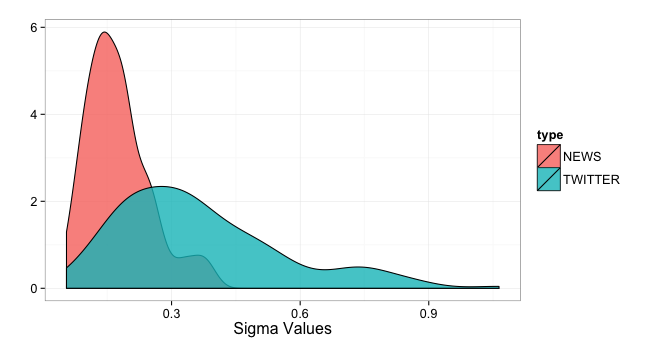
\includegraphics[width=.5\textwidth]{imgs/diff_sigma}
	\caption{Distribution of Sigmas}
	\label{fig:sig}
\end{figure}

While a host of comparisons could be made between the news and Twitter data we study, we restricted ourselves here to a subset of questions of particular interest. First, we are interested in the level of variance over time in discussions of particular themes in particular countries on Twitter as compared to in news.  Conveniently, our statistical model provides us with a parameter, $\sigma^2_{w,r}$ which captures the extent of this variability. Figure~\ref{fig:sig} shows a density plot detailing the distribution of values for $\sigma^2_{w,r}$ for the news and Twitter data.  As is clear, Twitter data is much more variable in the news, both in the average variability across a particular theme/country time series and with respect to the expected value of $\sigma^2_{w,r}$ in general.  This finding shows that news coverage of the Arab Spring was more stable than discussion on Twitter.  Our results correlate with the idea that while the propagation of content is similar in form in both Twitter and news media,  the social elements of Twitter introduce important variability in the diffusion and longevity of discussion \citep{yang_patterns_2011}.  Perhaps more importantly, our findings show that the extent to which a change in thematic focus is ``interesting'' differs when analyzing news versus Twitter data. Researchers using social media data to interpret change in social processes, our data suggests, must be more cautious than those with access to news data.

In addition to levels of variability in the two media, we are also interested in the extent to which news and Twitter data focused on the same topics at the same time.  That is, we are interested in the extent to which the time series of $\eta_{w,r,t}$ values for Twitter and news are correlated for a particular theme/country combination.  Importantly, this correlation cannot be measured directly with our $\eta_{w,r,t}$ - baked into our model is the assumption of autocorrelation with a one-month lag (Equation~\ref{eq:eta_eq}), which will lead to spuriously high correlation values.  To infer correlations between news and Twitter data, we therefore must remove the autocorrelation by subtracting the prior month's value from each activation score.  More specifically, for a given country $r$ and category $w$, we construct a vector of observations $\eta_{w,r,t}-\eta_{w,r,t-1} \quad \forall \, t > 1$ for both Twitter and news data. These vectors are, via the assumptions of our model, void of autocorrelation and can therefore be compared directly using, for example, a simple Pearson correlation.

The first question is whether or not there is a significant correlation between the news and Twitter across all countries and themes. Importantly, we would expect this correlation to be positive and significant for the non-stopword data, and to be close to zero for our stopword themes. Using the bootstrap procedure  with 10000 iterations, we construct 99\% confidence intervals using a pivot interval \citep{wasserman_all_2003} on the Pearson correlation between news and Twitter data. That is, we determine the extent to which the changes in activation from the previous month in Twitter data are linearly correlated with changes from the previous month in news data, taking as input all observations across all countries.  We perform this analysis twice, once for the non-noise (non-Stopword) themes and once for the noise-only themes.


The correlation for the non-noise data is .23 [.17,.28], indicating a moderate but significant correlation between news and Twitter.  There are several reasons for the existence of this correlation. Perhaps most importantly, it is well known that news agencies send tweets about their key stories, and retweets of these stories comprise an important component of discussion on Twitter. Thus news and Twitter should be correlated, as they form a part of a symbiotic media system.  In some sense, it is therefore interesting that the correlation between the two media is not higher.  One obvious reason is that personal, socially-focused discussions do of course occur on Twitter. Additionally, a large volume of tweets are known to be sent by bots on Twitter, many of which are just tweeting nonsense phrases.

The correlation for the noise-only data was .1 [-.001, .19].  Results suggest that correlations between non-noise themes is (significantly) greater than noise themes, and that the noise data was not significantly different from 0 at $\alpha=.01$. However, results do indicate that there may still be some level of correlation in the residual noise in our data between news and Twitter.  This may be due to a variety of factors, perhaps most obviously the fact that we treat each country independently.  While future work may consider means of addressing these biases, we instead choose here only to account for the possible existence of this spurious correlation when considering further results. We now turn to explore which themes had the strongest and weakest correlations between news and Twitter (across all countries). 

\begin{figure}
	\centering
	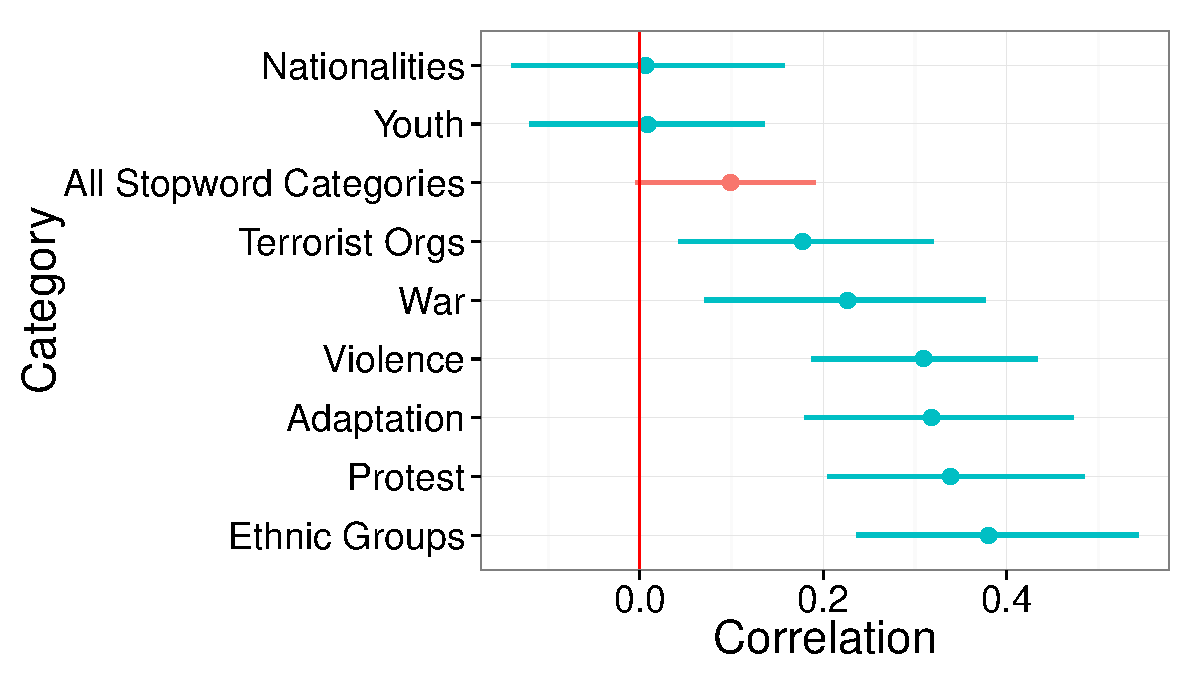
\includegraphics[width=.5\textwidth]{imgs/cat_corr}
	\caption{News/Twitter correlations by category.  Confidence intervals are 99\% bootstrapped CIs calculated with a pivot interval and 10000 iterations}
	\label{fig:cat_corr}
\end{figure}

Figure~\ref{fig:cat_corr} presents the correlations between news and Twitter data for each category, with data aggregated across countries. Additionally, we have aggregated all noise categories into a single category, entitled "All Stopword Categories".  Confidence intervals are constructed in the same way as above, and are shown in the figure via the lines for each category. Mean estimates are shown with a dot.  Figure~\ref{fig:cat_corr} shows that the strongest correlations between news and Twitter occur in reference to general indicators of revolution, specifically, protest and violence. The general level of correlation across these categories supports the idea that news and Twitter discussions specific to the revolution fed off of each other \citep{cottle_media_2011,comunello_will_2012}. Additionally, we can expect that this may be due to the fact that the Tweets by news agencies are focusing in this area. In addition, we observe strong correlations between media in discussions of adaptation and change and to ethnicity. 

On the other hand, in comparison to the Stopword categories,  there is no significant correlation\footnote{at a level of $\alpha=.001$ using the parametric test described in \citep{zou_toward_2007}} for discussions of national identity, youth movements, terrorist organizations and war.  With reference to the ``selecting on the dependent variable'' problem in social media research \citep{tufekci_big_2014}, our findings indicate that scholars focusing too heavily on particular topics may over or under-estimate the correlations between topical focuses of news and Twitter.  Perhaps most interesting is the fact that while discussion of Ethnic, or non-national, identities was highly correlated between the two media, discussion of national identities show little, if any, correlation between media  This difference is important in considering the extent to which news or Twitter data can be used to support the idea of an evolving national identity in contrast to factionalized identities, and suggests that the evolution of a national identity may be a factionated process that is not well monitored by using a single media source. Thus, in future study of \citeapos{goldstone_cross-class_2011} hypotheses on how the proliferation of national identity was important to the success of revolutions, one must consider both news media and Twitter separately in attempting to understand how the existence of a national identity played out in the media landscape surrounding the Arab Spring.   

\begin{figure}
	\centering
	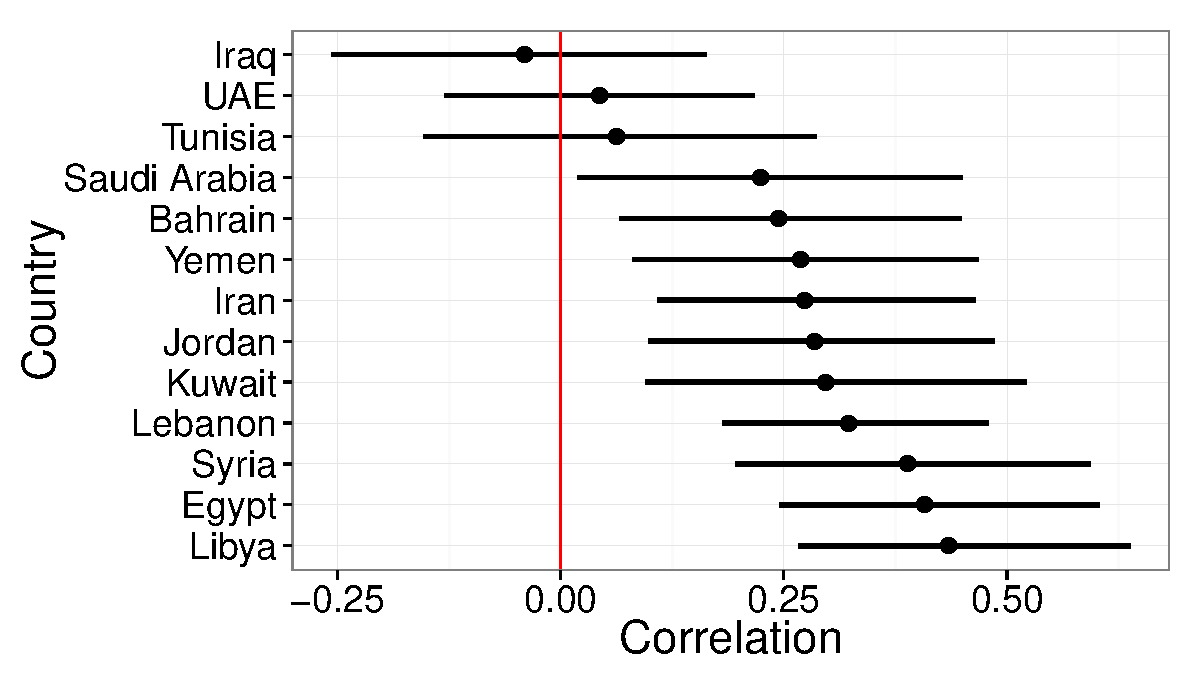
\includegraphics[width=.5\textwidth]{imgs/country_corr}
	\caption{News/Twitter correlations by country}
	\label{fig:corr_country}
\end{figure}

Finally, Figure~\ref{fig:corr_country}  shows correlations between news and Twitter across countries, aggregating across all non-noise themes.  Here, as there is no noise baseline to compare to, we only consider differences from zero in our interpretation.  In light of previous work, the most interesting point to be taken from Figure~\ref{fig:corr_country} is that countries where data has been compared across news and Twitter in the past differ in the ways in which news relates to Twitter. In particular, while there are high levels of correlation between news and Twitter in Libya, Syria and Egypt, no significant correlation exists between these two media in Tunisia.  This implicates the fact that consideration of a single country may also lead to biased conclusions on the relationship between news and Twitter during the Arab Spring. More specifically, it seems that in countries with sustained levels of civil unrest (Syria, Egypt and Libya), news and Twitter are more likely to converge on thematic discussions. In contrast, in countries like Tunisia, where the majority of the civil unrest was short-lived, thematic discussions appear to deviate between the two media. Similarly, correlations in nations where no massive government change occurred show only weak or non-existent correlations between the media.  This may be because in these countries the discussion in the news was on political, economic an global events, but in Twitter it focused on social, cultural and personal events.

\subsection{{\bf RQ2:} Relating to events on the ground}

\begin{table*}[t]
\centering
\begin{tabularx}{\textwidth}{|m{.3cm}| l| l| l| l| m{.7cm}|  X |}
  \hline
 N & Category & Country & Media & Date & +/- Change & Major Event \\ 
  \hline
1 & War & Syria & News & 3/2011 & - & Week of March 15-21 is considered to be the beginning of the Syrian uprising\footnote{\url{http://en.wikipedia.org/wiki/Syrian_Civil_War#Protests_and_armed_insurgency_.28July_.E2.80.93_October_2011.29}} \\   \hline
  2 & Protest & Syria & News & 3/2011 & + &Week of March 15-21 is considered to be the beginning of the Syrian uprising \\   \hline
  3 & Ethnic Groups & UAE & Twitter & 10/2012 & + & EU report condemning human rights climate in UAE \\   \hline
  4 & Protest & Tunisia & Twitter & 8/2012 & + & Tunisian women stage large protests\footnote{\url{http://www.aljazeera.com/indepth/features/2012/08/201281981854620325.html}} \\   \hline
  5 & War & Lebanon & News & 3/2011 &  - & Major rallies throughout the nation on various days\footnote{\url{http://en.wikipedia.org/wiki/2011_Lebanese_protests}}\\   \hline
  6 & Adaptation & Libya & Twitter & 8/2012 & + & First free elections were held in Libya in July, 2012   \\ \hline
  7 & Adaptation & Tunisia & Twitter & 10/2011 &  - & First free election in Tunisia since 1956\footnote{\url{http://en.wikipedia.org/wiki/Tunisian_Constituent_Assembly_election,_2011}} \\   \hline
  8 & Terrorist Orgs & Libya & News & 9/2012& + & Attack on U.S. consulate in Benghazi, Libya \\   \hline 
  9 & Terrorist Orgs & Egypt & Twitter & 11/2012 & + & Major protests in Tahrir Square and the beginning of Parliamentary Elections \\  \hline 
  10 & Adaptation & UAE & Twitter & 10/2012 &  - & EU report condemning human rights climate in UAE  \\ 
   \hline
\end{tabularx}
\caption{The top 10 most surprising changes in activation from the previous month.  The column ``+/- change'' indicates if the change was an increase or decrease in activation.  The column ``Major Events'' gives an explanation of the major events that occurred during that month or the previous month (as change is relative to the previous month), or none if no such event occurred.}
\label{tab:events}
\end{table*}

In this section, we explore the extent to which large, sudden changes in activation rates in particular theme/country pairs were indicative of important real-world changes occurring in the Arab world.  Table~\ref{tab:events} lists the ten most ``surprising'' jumps in terms of change in activation from one month to the next.  We ranked the extent to which events were surprising using absolute change in activation, controlling for the overall level of variance for a particular theme/country pair.  That is, for month $t$ in country $r$ for theme $w$, surprise was calculated as $\frac{|\eta_{w,r,t}-\eta_{w,r,t-1}|}{\sigma^2_{w,r}}$.  Table~\ref{tab:events} also shows whether the change was positive or negative (in the column ``+/- change'') and briefly details the major events we believe led to this change.  

Model output shows that the beginning of the Syrian Civil War had the strongest impact on news media. Discussion of war decreased significantly relative to the previous month, as reporters sought to cover the increasing volume and intensity of protests throughout the country. These events, of course, marked the beginning of a civil war that is still well under way (as of the time of writing), showing the model’s propensity to capture important changes in events via news media. In general, sizeable changes in news media’s topical coverage were relevant to emergent protests. Interestingly, this focus appears to manifest in our model as a decrease in discussion of war as opposed to an increase in the discussion of protest. That is, the shift of news coverage away from war or the possibility of war is as indicative of critical protest events as is discussion of the protests themselves. We will see that this effect is significant in interpreting news discussion with respect to Libya, as we explore in our case study. 

In contrast to news media, the most prominent events that caused observable large shifts on Twitter were elections. In Libya and Tunisia, elections led to differences in discussions of adaptation and change, a sign that these elections may have promoted an influx of hopeful discussion of a new era in these countries. In contrast, in Egypt, elections led to increased discussions on organizations with known connections to terrorism, for example, the Muslim Brotherhood or al-Qaeda. The difference in thematic focus in these different elections is an important implication of the differences regarding sentiments towards the elections in each country, and something of interest to future work In addition to elections, the gender equality protests in Tunisia, staged heavily on social media \citep{yuce_womens_2015}, appear as a signal in the Twitter data but not in the news data.  

Finally, with respect to the Twitter data, two entries relating to the UAE in Table~\ref{tab:events}, both of which are relevant to the publication of a European Union report condemning human rights conditions for certain ethnic groups in the country, show up as events which captured a surprising level of discussion relative to the general level of focus on the themes of ethnic identity and adaptation to change in the UAE. Similarly, in the news data, a surprising level of discussion focuses on the attack of a U.S. consulate in Benghazi, Libya.  These issues were relatively minor with respect to their implications for the Arab Spring, but relatively major with respect to the interest drawn to them by U.S. and U.K. media.  The change in discussion that resulted from these events is thus a reminder that the Western-media centric data utilized for this study presents a possible roadblock in 


	\subsection{{\bf RQ1}: News vs. Twitter}
	\input{compare_to_overthrow}
	
\section{Case Study}

Our case study is divided into two sections. In the first, we focus on understanding how countries cluster in thematic space, particularly with respect to protest. In the second, we consider in greater detail how patterns in the protest theme differentiated by media provide support for claims explored by \cite{cottle_media_2011}.

\subsection{Connecting countries and themes}

\begin{figure*}[th]
	\centering
	\begin{tabular}{cc}
		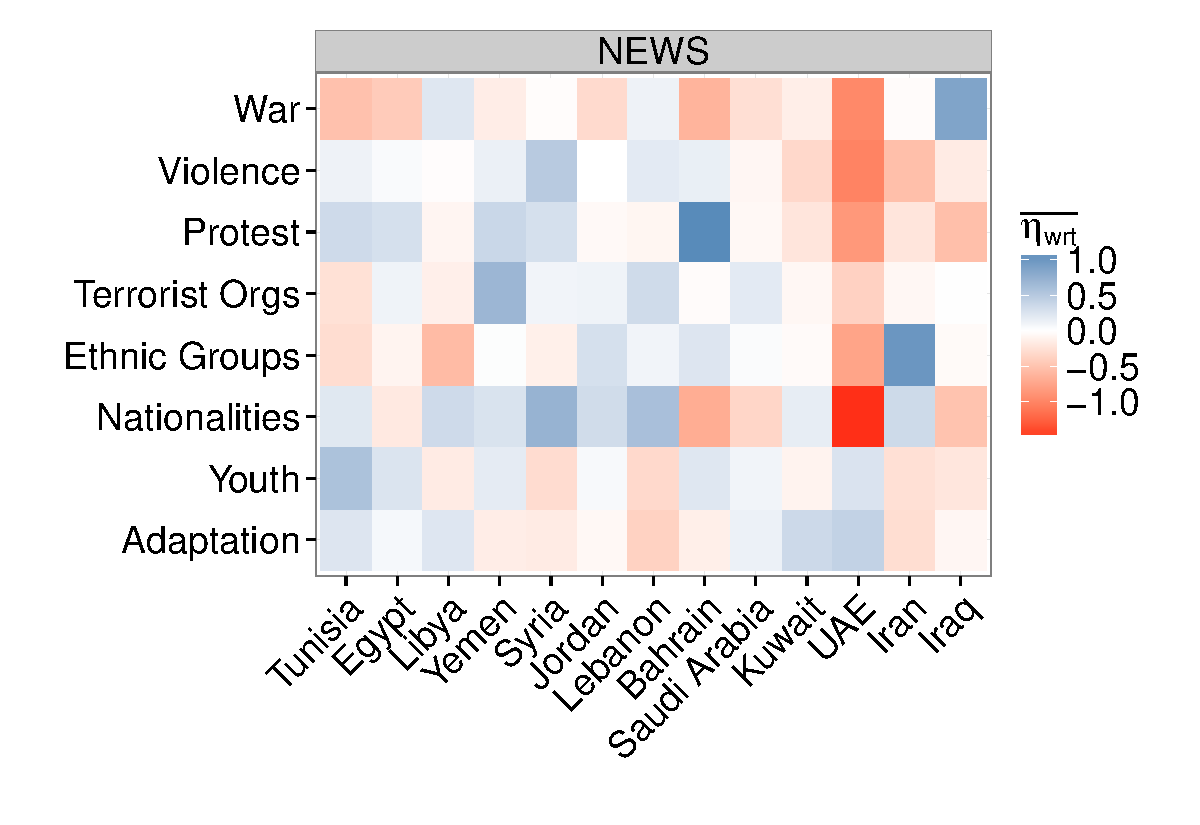
\includegraphics[width=.5\textwidth]{imgs/activity_topics_news} &
		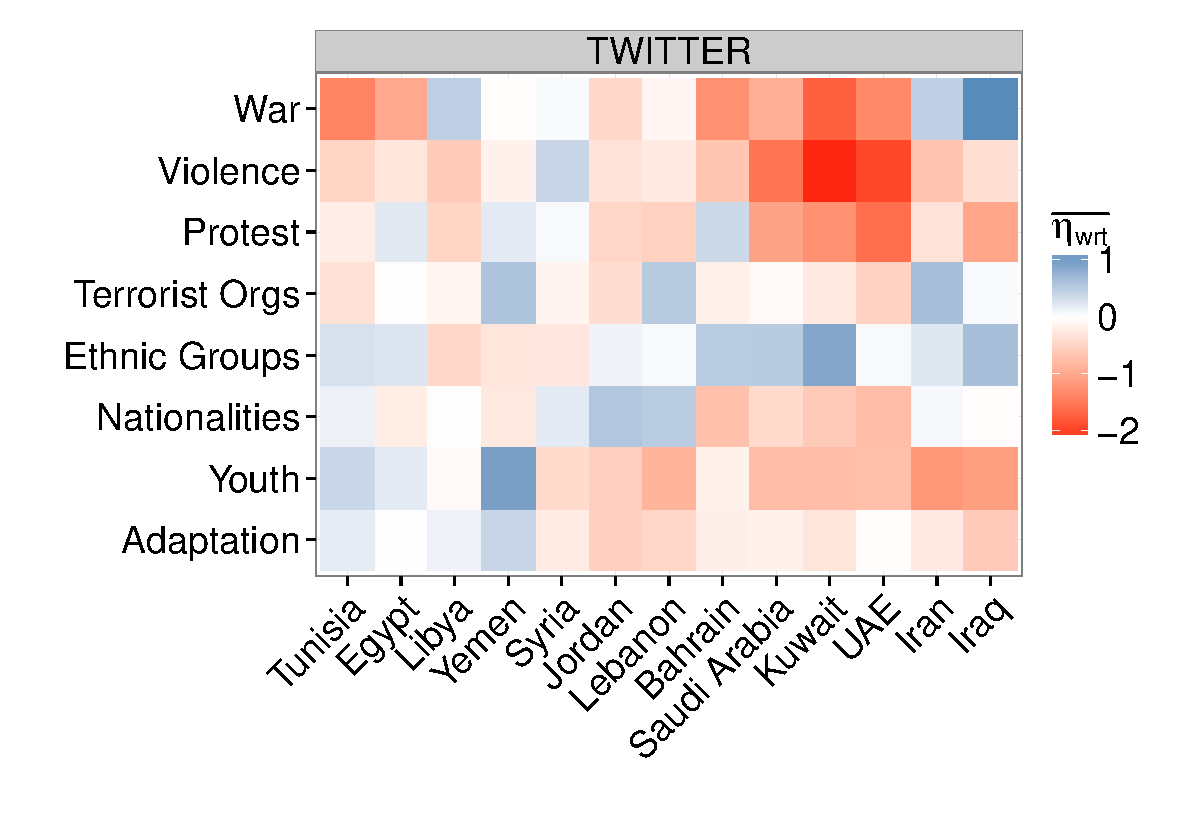
\includegraphics[width=.5\textwidth]{imgs/activity_topics_twitter} \\
	\end{tabular}
	\caption{Mean activation rate over all months for each country and category combination.  The higher the value above 0, the darker the blue. The lower the value below 0, the darker the red. }
	\label{fig:overall}
\end{figure*}


Figure \ref{fig:overall} shows two plots, one for news (left) and one for Twitter (right). Each plot depicts a heatmap of the mean activation values ($\overline{\eta_{w,r,t}}$) over all months for each country/theme combination. The higher the mean activation score above zero for a particular theme/country combination, the darker blue the square. The lower the value below zero, the darker the red. Additionally, note that values are interpretable relative to global activity of each topic/country combination. That is, the dark blue square in the top right of the Twitter plot shows that, on average, relative to other countries, discussions of war were more frequent in Iraq than the discussion of other topics. 

Figure \ref{fig:overall} suggests two fascinating patterns in how countries clustered along themes explored here. First, we considered how countries clustered along perhaps the most interesting theme with respect to the Arab Spring, that of protest.  Figure~\ref{fig:overall} shows that for countries in which protests occurred at relatively low levels (Iran, Iraq, Saudi Arabia and the UAE), discussion of protests were low in both the news and Twitter data. Interestingly,  however, even in countries where relatively high levels of protest occurred, a distinction can be made in the level of discussion of protest between countries where revolutions are still ongoing or succeeded in overthrowing the government (Egypt, Yemen, Tunisia, Libya, Bahrain and Syria) versus those where little social change occurred (Jordan, Kuwait, Lebanon).  In all but Libya, countries where social change followed protests showed positive (above zero, on average) levels of discussion about protest in the news media data. In contrast, countries where protests failed to produce significant results showed negative activation rates for this theme, on average, across time.  In the Twitter data the same patterns hold, although discussion of protest in Tunisia, who's government fell before the beginning of our data collection, is also negative.

\begin{figure}[t]
	\centering
	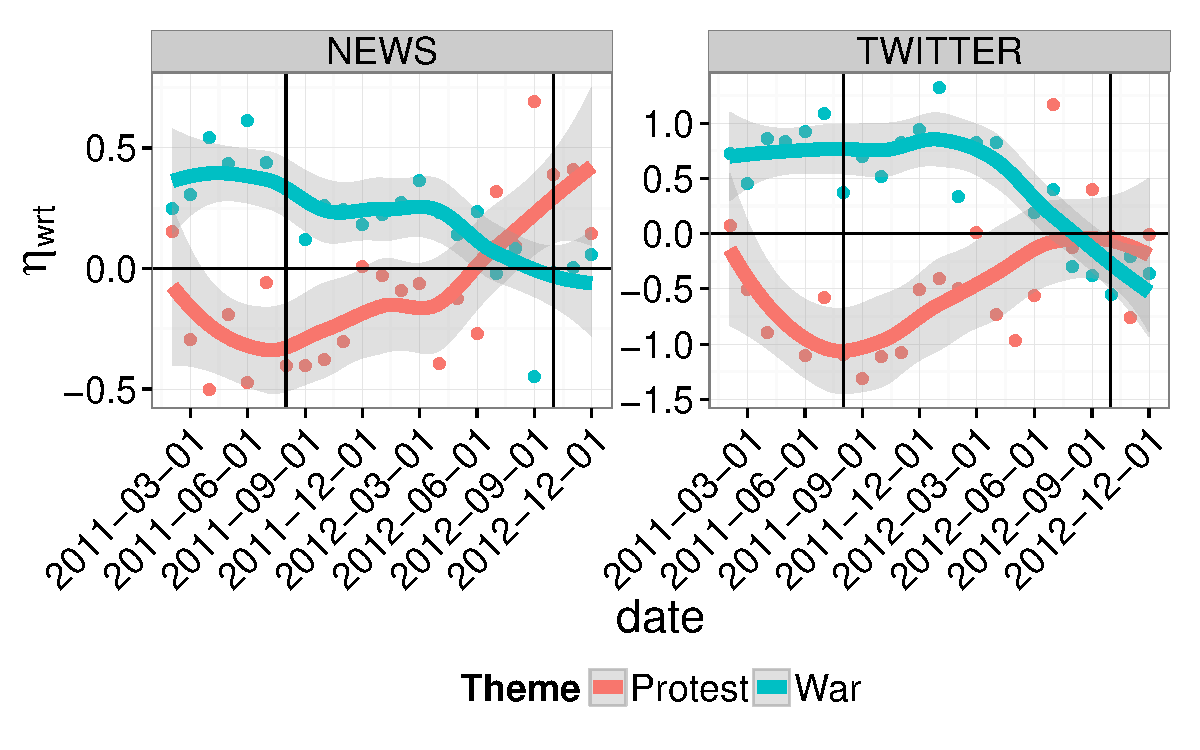
\includegraphics[width=.5\textwidth]{imgs/lib_protest_viol}
	\caption{Relationship between the protest and war themes over time in Libya. Points represent estimates from the model, nonparametric smoothed estimates with 95\% confidence intervals are provided as lines to ease visual observation of trends.}
	\label{fig:prot_viol}
\end{figure}

In sum, results show that in both Twitter and news media, levels of discussions about protest clustered into countries in which important social change occurred during the period, where positive activation scores for protest were observed, and countries where little or no social change occurred, where negative activation scores were seen. The lone exception to this categorization was Libya, where a six month civil war eventually led to the downfall of the ruling regime. We can understand why low levels of discussion on the subject of protest occurred by looking at the way in which protest was discussed over time in Libya. Figure~\ref{fig:prot_viol} shows the activation rates of the categories protest and war over time in Libya. The first vertical black line represents, approximately, the point at which the ruling regime was overthrown, the second black line represents the attack on the U.S. consulate in Benghazi.  As we can see, the focus in Libya on protest may largely have been mediated by a focus on the civil war and its aftermath.  However, as unrest grew again in the face of complaints about the new regime, we do see a renewed trend towards protest, which could be seen as an initial indicator of a return to civil unrest.  This intricate relationship between discussions of war and protest is of particular interest in understanding how unrest leads to organized violence.
 
\begin{figure}[t]
	\centering
	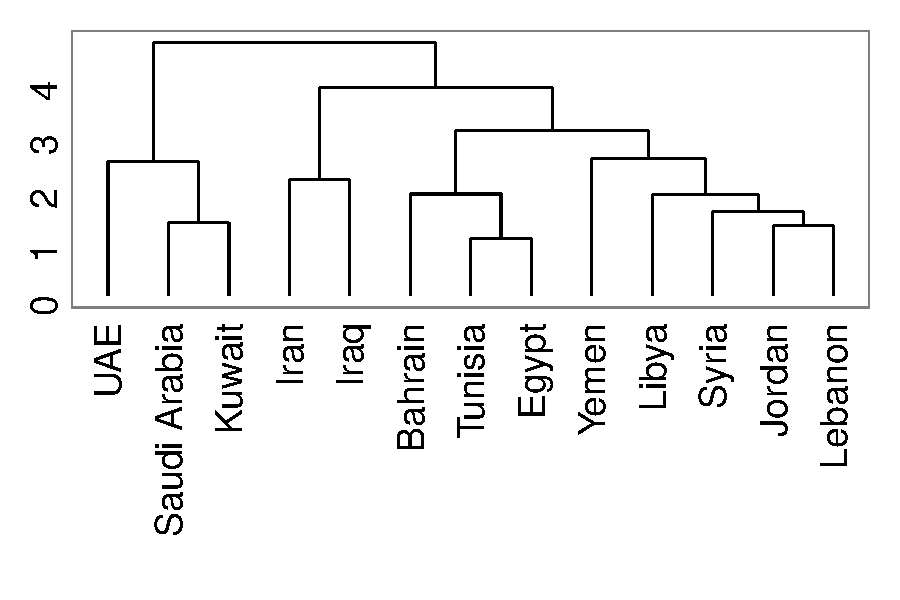
\includegraphics[width=.5\textwidth]{imgs/country_dendro}
	\caption{Hierarchical clustering of our 13 countries based on mean activation levels across all categories for both news and Twitter }
	\label{fig:clust}
\end{figure}

Figure~\ref{fig:overall} also suggests there exists clusters of countries that exist at a larger level than simply distinctions across protests.  To better evaluate the extent to which this clustering exists, we perform a standard, complete-linkage, agglomorative clustering, where each country is represented by sixteen features (the eight categories shown in Figure~\ref{fig:overall} for both news and Twitter). Figure~\ref{fig:clust} presents a dendrogram of the resulting clustering.  Figure~\ref{fig:clust} shows that the oil-rich nations of Saudi Arabia, Kuwait and UAE, where little social change occurred, showed similar thematic structures.   Similarly, nations with which the United States has the strongest tensions, Iran and Iraq, cluster together.  Figure~\ref{fig:clust} shows that these five countries  are heavily separated in thematic content from nations where social change occurred, although they are also separated from perhaps the more similar nations of Lebanon and Jordan.  Within the cluster holding nations where large-scale social change occurred, we observe that Tunisia and Egypt are the most tightly connected, an indication of the extent to which these two revolutions were tied together. 

\subsection{Temporal patterns in protests}

\begin{figure}[t]
	\centering
	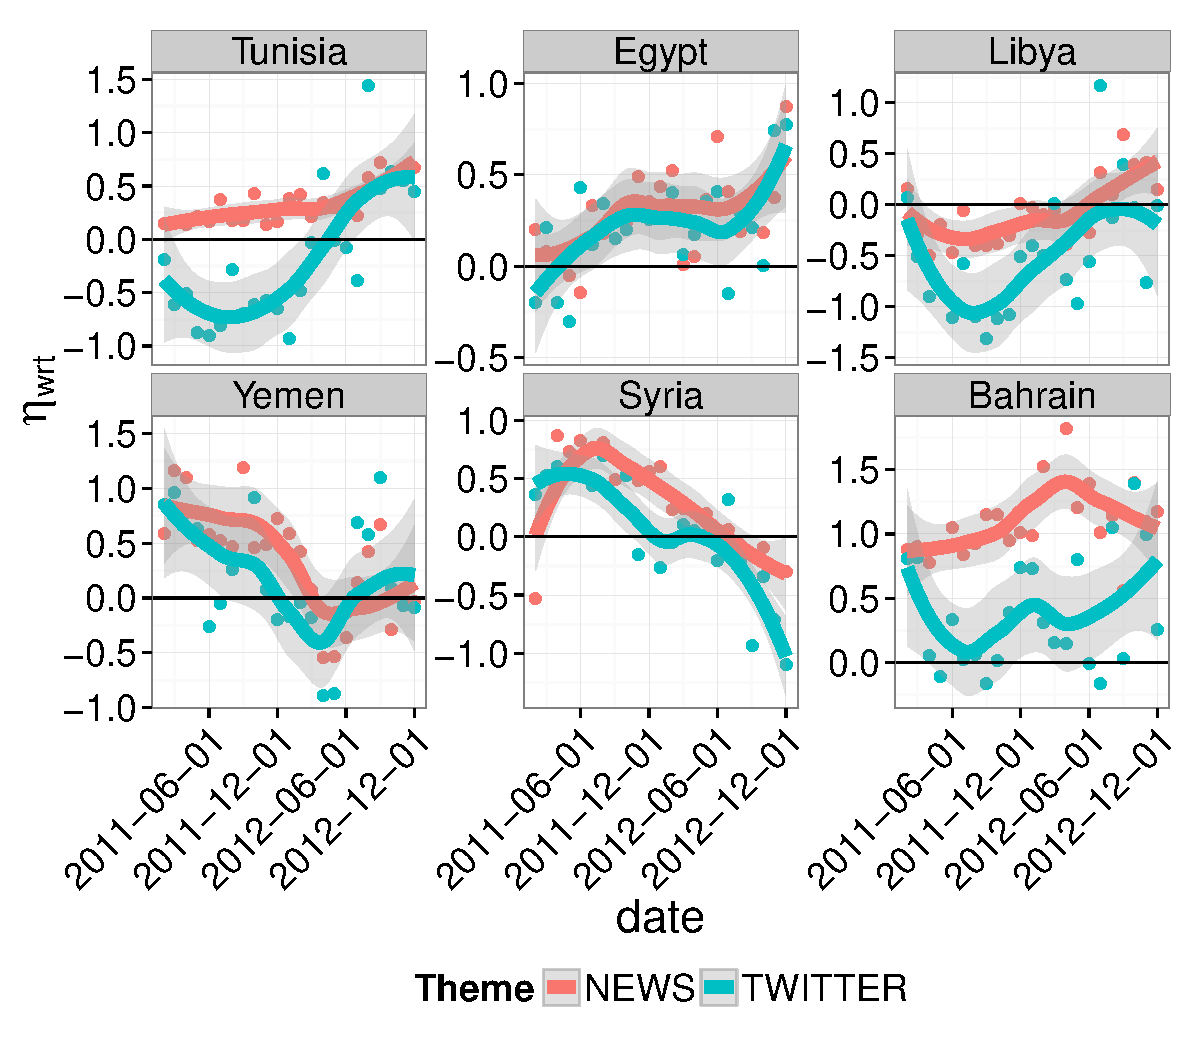
\includegraphics[width=.5\textwidth]{imgs/cottle}
	\caption{Activation Rates of protest over time for six countries of interest.  Points represent estimates from the model, nonparametric smoothed estimates with 95\% confidence intervals are provided as lines to ease visual observation of trends.}
	\label{fig:cottle4}
\end{figure}

Having noted that important clustering appears in average levels of activation with respect to protests, we turn now to how temporal patterns of protest played out in both news and Twitter for nations where high levels of social change occurred. Figure~\ref{fig:cottle4} illustrates activation rates for the theme of protest in news media and Twitter for Bahrain, Egypt, Libya, Syria, Tunisia and Yemen. Our findings, even over time, are consistent with the idea presented by \cite{cottle_media_2011} that new media played an important role in discussions of protests during the Arab Spring.  Perhaps more interestingly, \cite{cottle_media_2011} also argues that the relationship between social media and news media facilitated international recognition and protest legitimization, and provided human rights surveillance.  Our analysis is consistent with this assertion.  In contrasting results for Egypt, with its partially free press, to more restricted countries like Syria, Tunisia, and Bahrain, we observe that states with more oppressive regimes tend to show less of a relationship between social and news media. However, even in the more oppressive regimes, uptakes in Twitter activation with respect to protest always lead to corresponding changes in news activation rates which implies a strong interaction between the two media types. This relationship between news media and social media activation rates reinforce \citeapos{cottle_media_2011} premises. 

Since these clusters of countries we extract in this section are based on both news and Twitter, they cannot be attributed to just a western view of similarity among the countries.  Rather, they reflect some underlying commonality in the way information about and from the these countries is presented across a diverse media landscape.  On the one hand, these clusters show which countries have a common media profile and so, to an extent, a common pattern of media usage by the population.  On the other hand, these clusters may indicate how countries might be similarly influenced by a media campaign.  

%we pr little quantitative research exists analyzing the interaction between news and social media throughout the Arab Spring.   \citet{cottle_media_2011} presents the most comprehensive study to date and presents well argued hypotheses pertaining to the complex interactions between the two types of media and their implications for social change in MENA.  However, he does so with little empirical evidence and calls for ``careful documentation and comparative analysis in the months and years ahead.''  The following section will highlight how activation rates support or refute several of his assertions. 

%\todo{develop fig:cottle4. Decription: topic: protest countries: Bahrain, Egypt, Libya, Syria, Tunisia, Yemen. That depicts smoothed activation rates over time.  Similar to the blah2 plots}

% \todo{ I was not able to show a relationship between news v twitter correlation with either freedom of the press index or internet saturation.  I think there are a couple observations making this problematic.  First, very small set.  Protest and violence are only relatively important topics in a few countries, and not all of them are of equal interest in english speaking news media. I'm open to suggestions}


%	
%	\begin{figure*}
%		\centering
%		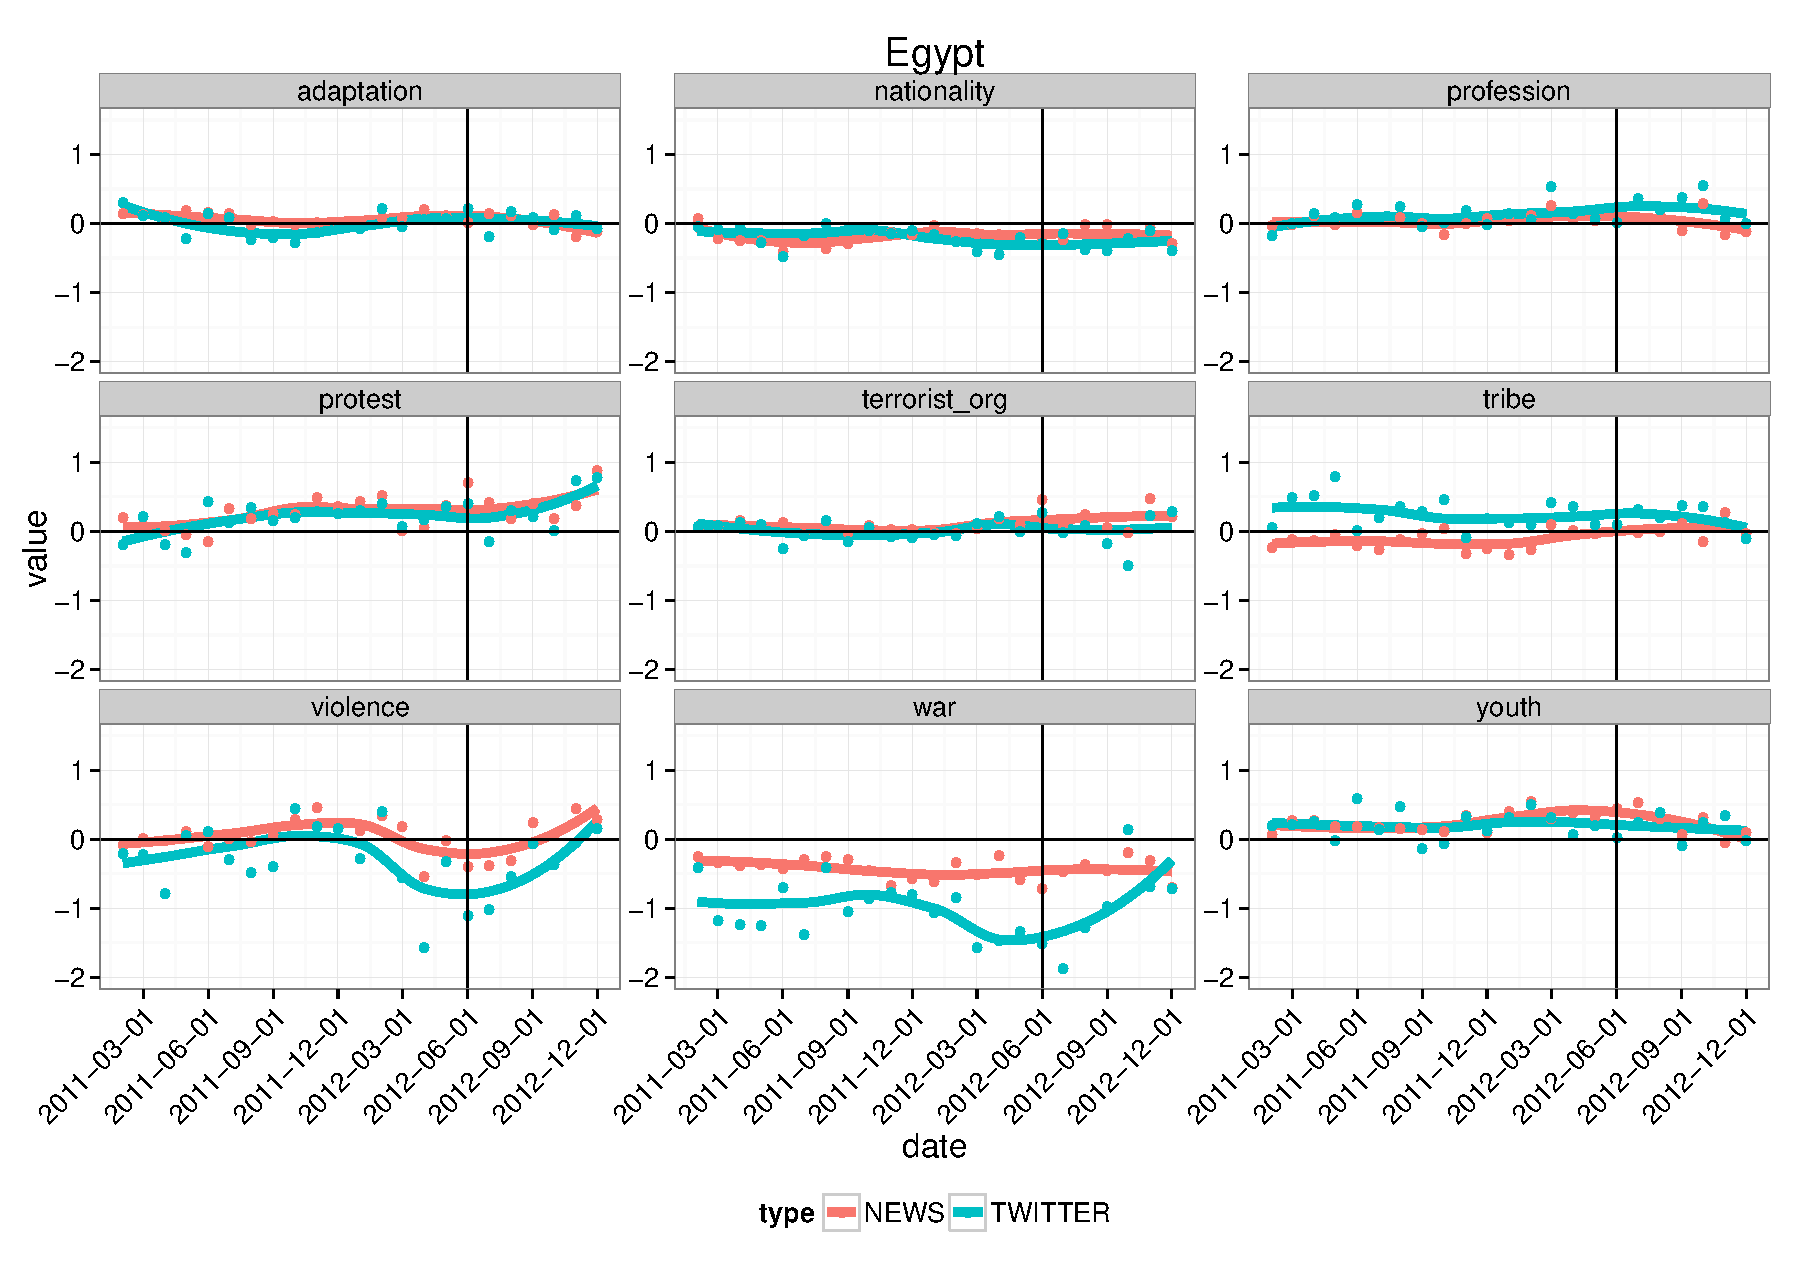
\includegraphics[width=\textwidth]{imgs/egypt.pdf}
%		\caption{Egypt: Black line is when Morsi is elected}
%		\label{fig:egypt}
%	\end{figure*}
%	
%	\begin{figure*}
%		\centering
%		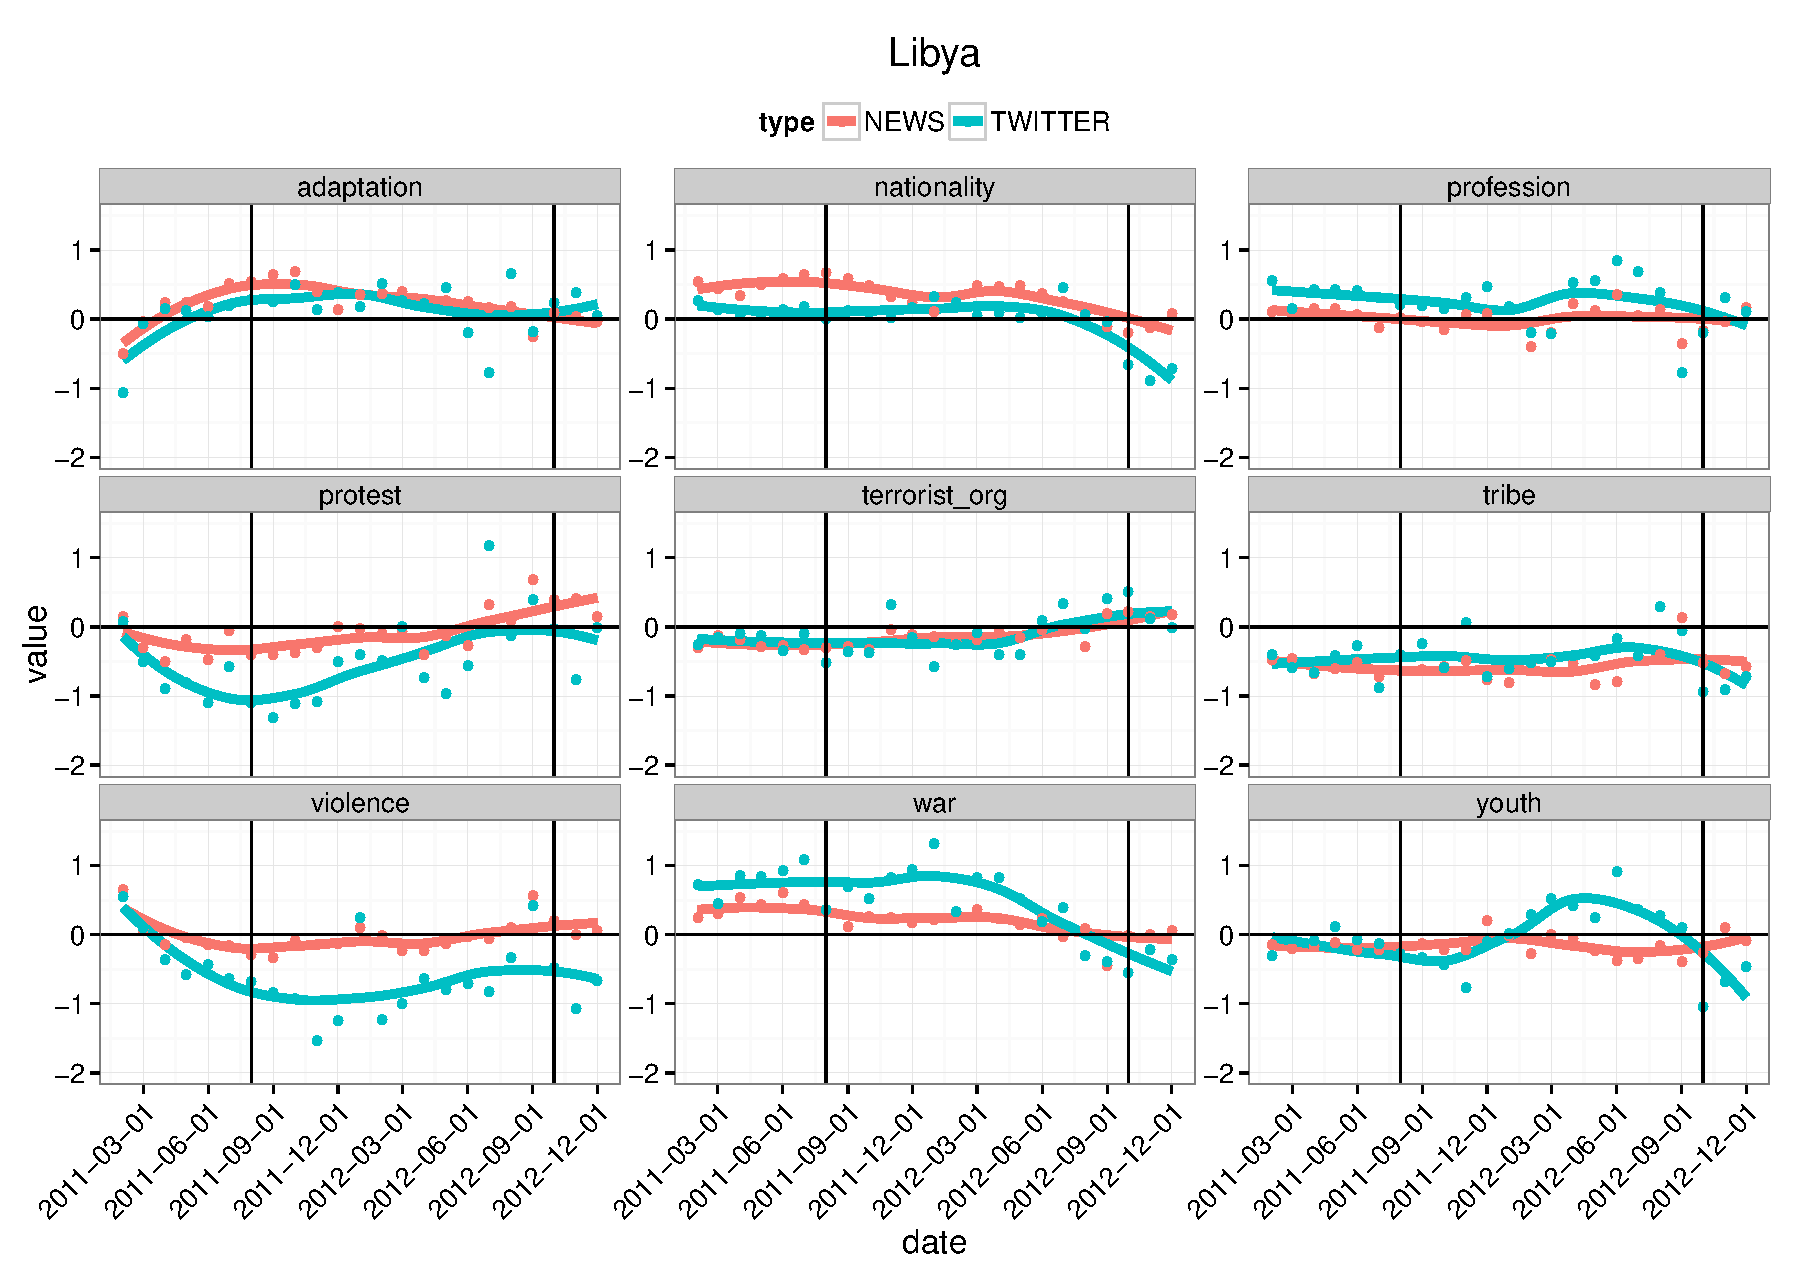
\includegraphics[width=\textwidth]{imgs/libya.pdf}
%		\caption{Libya: Black lines are death of Gaddafi and Benghazi }
%		\label{fig:libya}
%	\end{figure*}
%	
%	\begin{figure*}
%		\centering
%		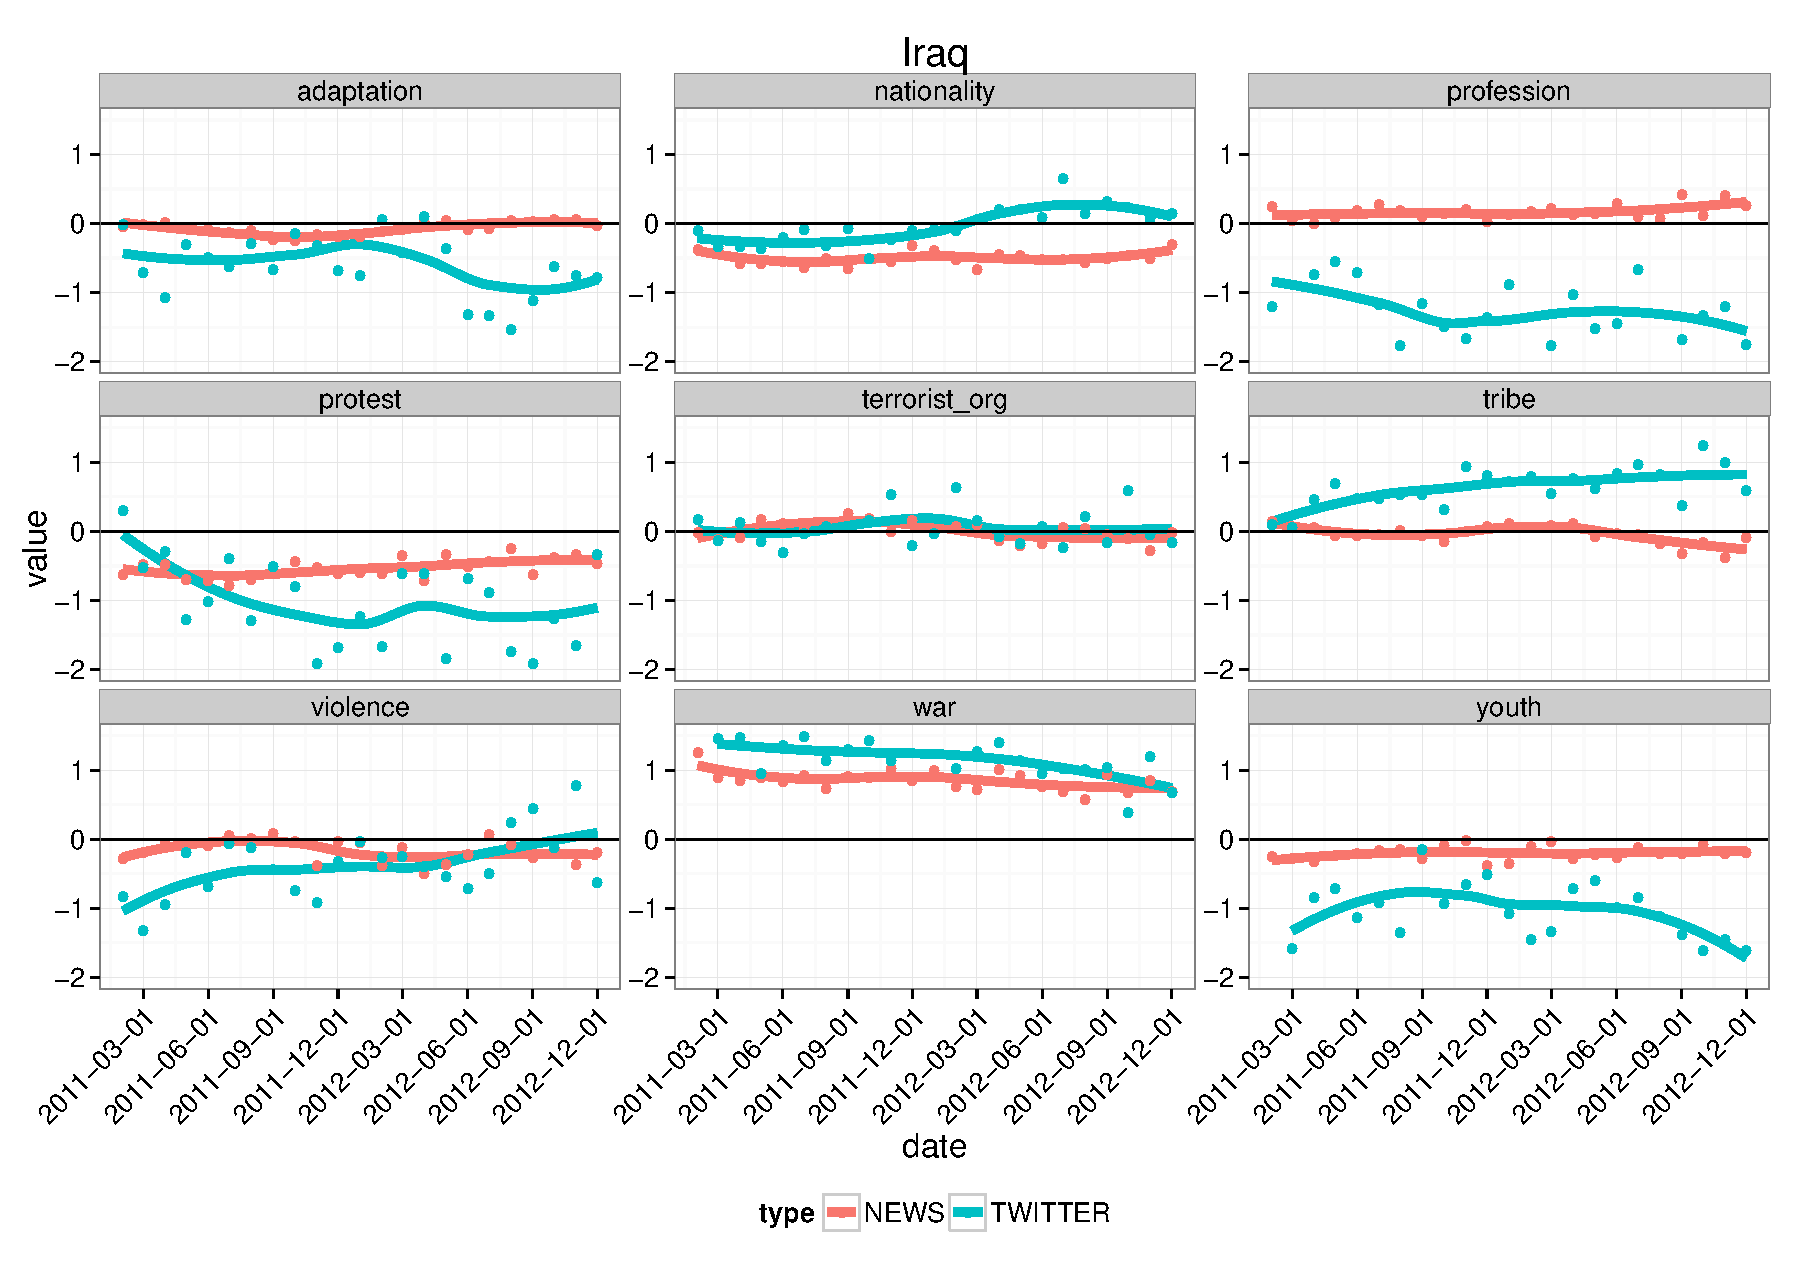
\includegraphics[width=\textwidth]{imgs/iraq.pdf}
%		\caption{Iraq}
%		\label{fig:iraq}
%	\end{figure*}
%	
%	
%	\begin{figure*}
%		\centering
%		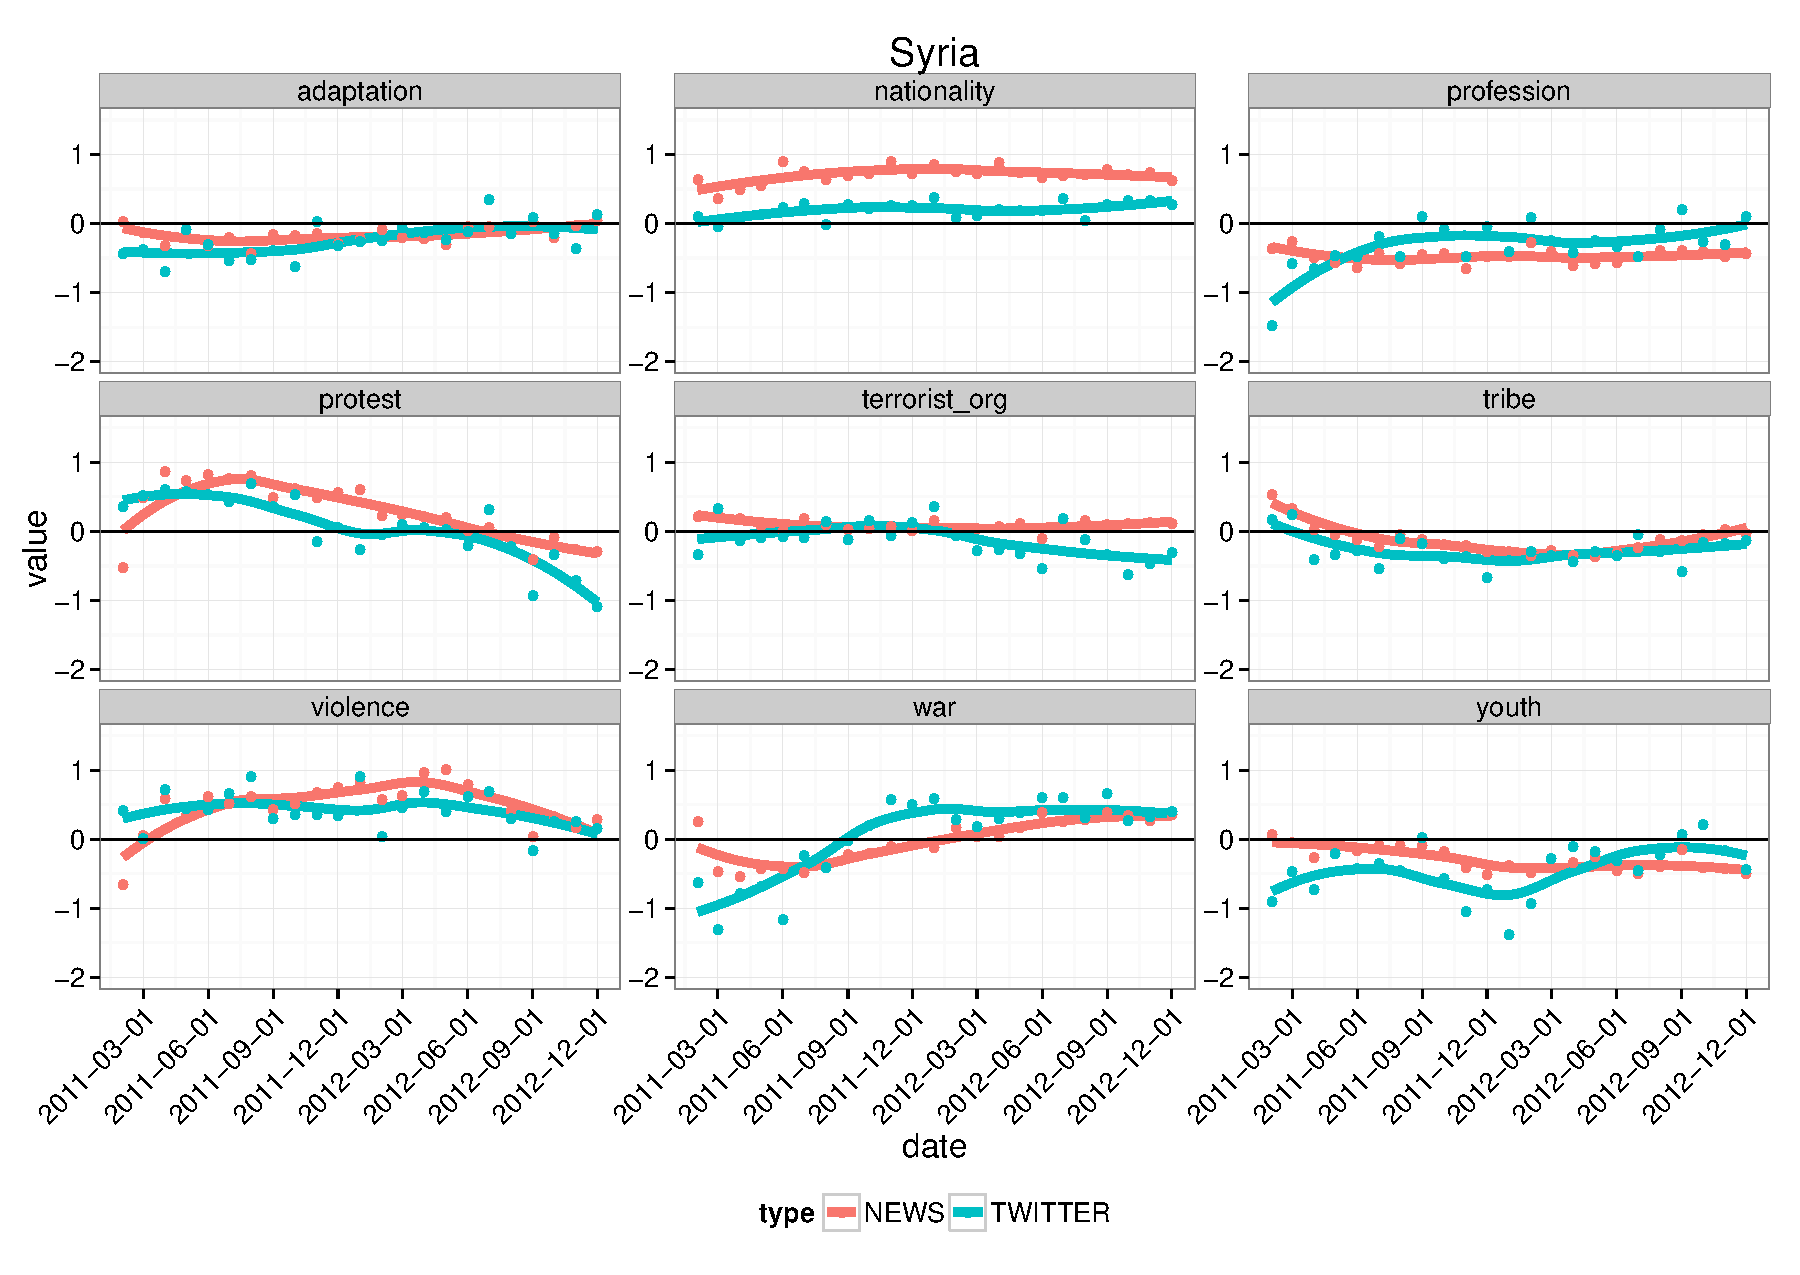
\includegraphics[width=\textwidth]{imgs/syria.pdf}
%		\caption{Syria}
%		\label{fig:syria}
%	\end{figure*}
%	 







\section{Conclusion}

Our analysis is cowith the acknowledgement of the rash of recent claims over the methodological trapdoors that exist within this type of data \cite{tufekci_big_2014,ruths_social_2014,joseph_approach_2014,morstatter_is_2013}. While these issues are not to be ignored, the present work utilizes cautious, nuanced analysis techniques which account for, or at least admit, these possible biases. 


\bibliographystyle{apa}
\bibliography{mybib} %your bib file


\end{document}
